\chapterimage{head2.png} % Chapter heading image
\chapter{Introduction}
\label{ch:introduction}
Nature's change and evolution is produced by the dynamics of the bodies and systems contained within the Universe. All the interactions of Universe can be described in terms of the four Fundamental Forces: gravitation, weak, electromagnetic and strong in ascending order of relative strength. High Energy Physics was able to unify the weak, electromagnetic and strong forces in terms of a $SU(3)\times SU(2)\times U(1)$ symmetry group in what is known as the {\it Standard Model} \cite{halzen1984quarks,peskin1995introduction,weinberg1995quantum,weinberg1996quantum,2000hep.ph....1283N}. Nevertheless, attempts to unify Gravitation with the other forces has still not provided satisfactory results.
\newline

The current consensus theory of gravitation is Einstein's General Relativity, that describes gravity as a universal deformation ($h_{\mu\nu}$) of the Minkowski metric tensor ($\eta_{\mu\nu}$)
\begin{equation}
g_{\mu\nu}(x^\lambda) = \eta_{\mu\nu}+h_{\mu\nu}(x^\lambda),
\end{equation}
where $g_{\mu\nu}$ is the metric tensor of the Universe. Gravity is postulated as a massless spin-two field with self-interaction Lagrangian
\begin{equation}
\mathcal{L}[g_{\mu\nu}] = \frac{c^4}{16\pi G_N}\sqrt{-g}g^{\mu\nu}R_{\mu\nu}(g),
\end{equation}
that couples minimally and universally to all the fields of the Standard Model; where $R_{\mu\nu}$ is the Ricci tensor, $c$ the speed of light and $G_N$ Newton's constant \cite{PhysRev.138.B988,feynman1995feynman,1969ApJ...157..857F,PhysRevD.33.3613,0264-9381-4-5-024,0264-9381-4-5-025,Olive:2016xmw}.
\newline

From the total action, Einstein's equation of the gravitational field can be obtained \cite{ANDP:ANDP19163540702,1916AnP...354..769E}:
\begin{equation}
R_{\mu\nu}-\frac{1}{2}Rg_{\mu\nu} = \frac{8\pi G_N}{c^4}T_{\mu\nu},
\label{eq:einsteinbare}
\end{equation}
where $T_{\mu\nu}$ is total energy-momentum tensor, that is the source of gravity.

\section{The expanding Universe}
\begin{figure}
\begin{center}
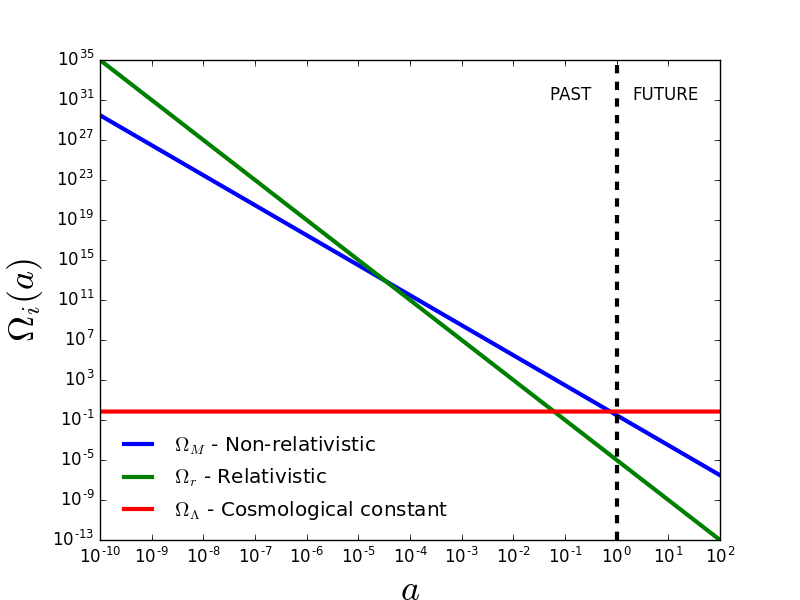
\includegraphics[width=0.75\textwidth]{./Pictures/rho_a.png}
\caption{Critical energy density for different types of matter species as function of the scale parameter of the Universe: relativistic (cold matter), non-relativistic (radiation), and cosmological constant. It can be seen that at present (black-dashed line), cosmological constant has just started to be dominant over the other species, starting the accelerated expansion era.}
\label{fig:rho_de}
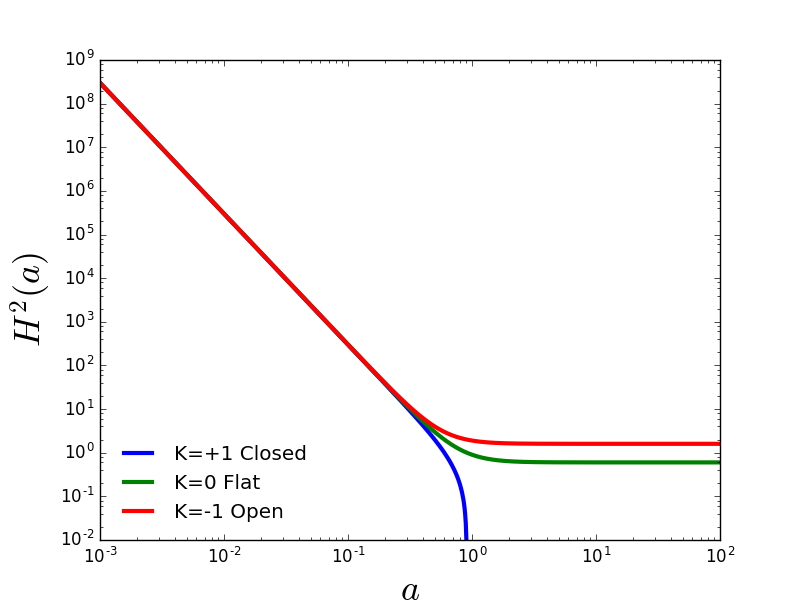
\includegraphics[width=0.75\textwidth]{./Pictures/scale_factor.png}
\caption{Expansion rate as function of the scale parameter of the Universe for different geometries (assume $\Omega_M=1$). The flat geometry expansion rate decreases until at infinity reaches zero. Open geometries show a constant expansion rate leading to an exponential growth of the scale factor. Closed geometries drops to zero very fast an eventually becomes negative leading to a re-collapse of the Universe.}
\label{fig:scale_geometry}
\end{center}
\end{figure}
One of the consequences of Einstein's equation is that the metric tensor is not static, implying that the geometry of the Universe changes. Thus, the Universe is a dynamical entity itself and its past and future evolution can be computed withing the framework of General Relativity.
\newline

Assuming that the Universe is homogeneous and isotropic \citep{2014MNRAS.440...10A,2015MNRAS.449..670A}, the only possible metric tensor is the Friedman-Lema\^itre-Robertson-Walker metric (FLRW) given by the line element \cite{1927ASSB...47...49L}
\begin{equation}
ds^2 = -dt^2+a^2(t)\left[\frac{dr^2}{1-Kr^2}+r^2(d\theta^2+\sin^2\theta d\phi^2)\right],
\end{equation}
where $a(t)$ is a function of time know as scale factor, $K=-1,0,1$ is the curvature of the universe and $r,\theta,\phi$ are spatial 3D spherical coordinates.
\newline

Solving Einstein's equation for this metric, an expression for the evolution of the scale factor with time can be obtained
\begin{equation}
H^2(t)\equiv \left[\frac{\dot a(t)}{a(t)}\right]^2 = \frac{8\pi G_N}{3c^4}\rho(t) -\frac{K}{a^2(t)},
\end{equation}
where the dot denotes time derivatives, and $\rho$ is the total density of energy. The parameter $H$ has been defined as the expansion rate and its value at present $H_0$ is known as Hubble's constant.
\newline

Expansion rate can be expressed in terms of the critical energy density
\begin{equation}
H^2(t) = H_0^2\left[\sum_i\Omega_i(t)-\Omega_K\right]
\label{eq:flrw}
\end{equation}
with
\begin{equation}
\Omega_K\equiv\frac{K}{[a(t)H_0]^2}\ \ \mbox{ and }\ \ \Omega_i(t)\equiv \frac{8\pi\rho_i(t)}{3H_0^2}.
\end{equation}
The parameter $\Omega_i$ is the critical density of the $i$-th matter/energy specie whose evolution with time can be computed using Thermodynamics. For non-relativistic matter --that is, matter with velocity $v\ll c$--, 
\begin{equation}
\Omega_M(t) = \Omega_M^0a^{-3}(t),
\end{equation}
whereas for relativistic matter species --that is, $v\sim c$-- also known as radiation,
\begin{equation}
\Omega_r(t) = \Omega_r^0 a^{-4}(t).
\end{equation}
Here $\Omega_i^0$ denotes the value on the present day of the $i$-th matter specie and by construction
\begin{equation}
\sum_i\Omega_i^0=1+\Omega_K
\label{eq:conservationenergy}
\end{equation}
\newline

Taking into account that the matter species and the curvature evolve on a different manner with time (\autoref{fig:rho_de}), its relative abundance at present fixes the expansion rate for the whole history of the Universe from birth to death. Discarding the hypothesis of empty Universe\footnote{At least, this Thesis is present at the Universe, therefore it is not empty.} and taking into account that for $a\rightarrow\infty$ all the matter species are diluted, three scenarios of expansion history can be considered depending on the curvature density of the Universe (\autoref{fig:scale_geometry}):
\begin{itemize}
\item {\bf Big Crunch:} Universe closed, with positive curvature ($K=1$). The attractive gravitational self-interaction of the Universe causes the gravitational collapse of the whole Universe into a single point.
\item {\bf Big Rip:} The Universe has negative curvature ($K=-1$), the gravitational repulsive self-interaction of the Universe causes a perpetual accelerated expansion.
\item {\bf Big Freeze:} The Universe is flat ($K=0$) and expands forever at a decelerated rate until it stops at $a\rightarrow\infty$.
\end{itemize}

Thus, the curvature of the Universe is the critical parameter to determine its thermal history. The latest combination of different cosmological probes determine it to be $\Omega_K = -0.0001^{+0.0054}_{-0.0052}$ \cite{2015arXiv150201589P}, quantity close to the floor of experimental accuracy \cite{2016PhRvD..94b3502L}, allowing to assume safely that the Universe is flat. Thus, the Universe is expected to be expanding at a decelerated rate. Although, the expansion of the Universe has been known for a century since Hubble's measurement of the recession velocity of galaxies \cite{1929PNAS...15..168H}, measurements of type-Ia supernovae (SNIa) two decades ago and  confirmed since then by several probes \cite{2008ARA&A..46..385F} show that the expansion of the Universe is accelerating (\autoref{fig:sdss_flatness} and \autoref{fig:sarkar_SNIa}).
\begin{figure}
\begin{center}
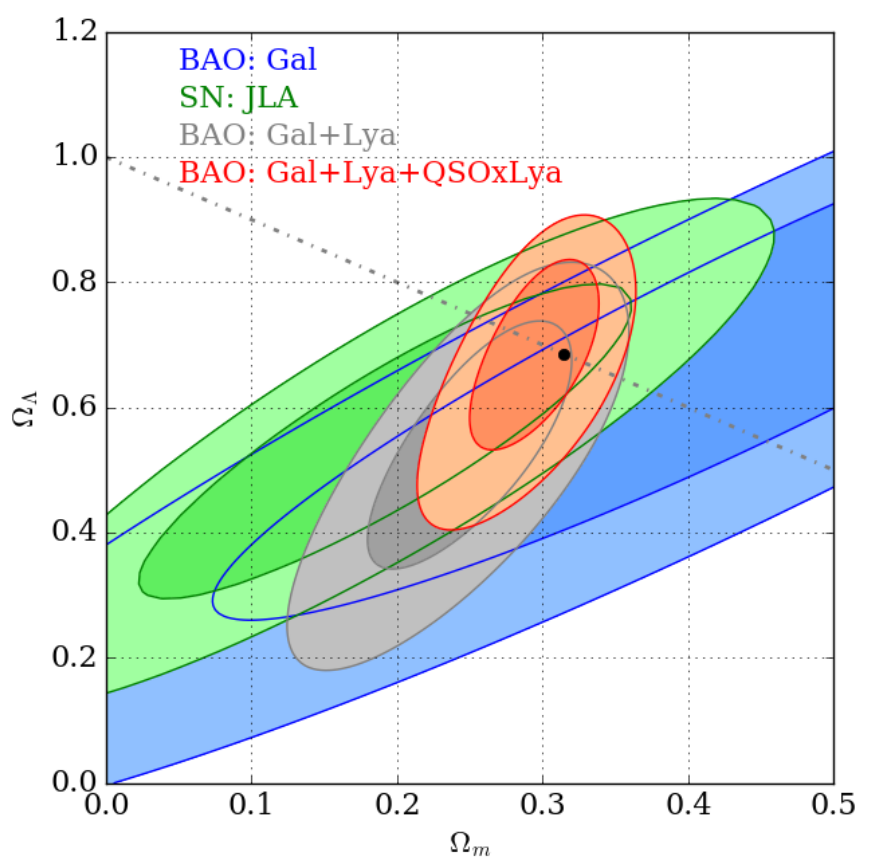
\includegraphics[width=0.7\textwidth]{./Pictures/omega_K_sdss.png}
\caption{Latest constrains on the curvature of the Universe measured by the combination of barion acoustic oscillation (BAO) and supernovas (SN) \cite{2017arXiv170200176B}. Curvature can be obtained with \autoref{eq:conservationenergy} assuming that the matter species are only dark energy and non-relativistic matter, $\Omega_\Lambda,\Omega_M$ respectively. Black-solid dot is Planck 2015 best-fit result \cite{2015arXiv150201589P}. Flat Universe is the dash-dotted line.}
\label{fig:sdss_flatness}
\vspace*{0.3cm}
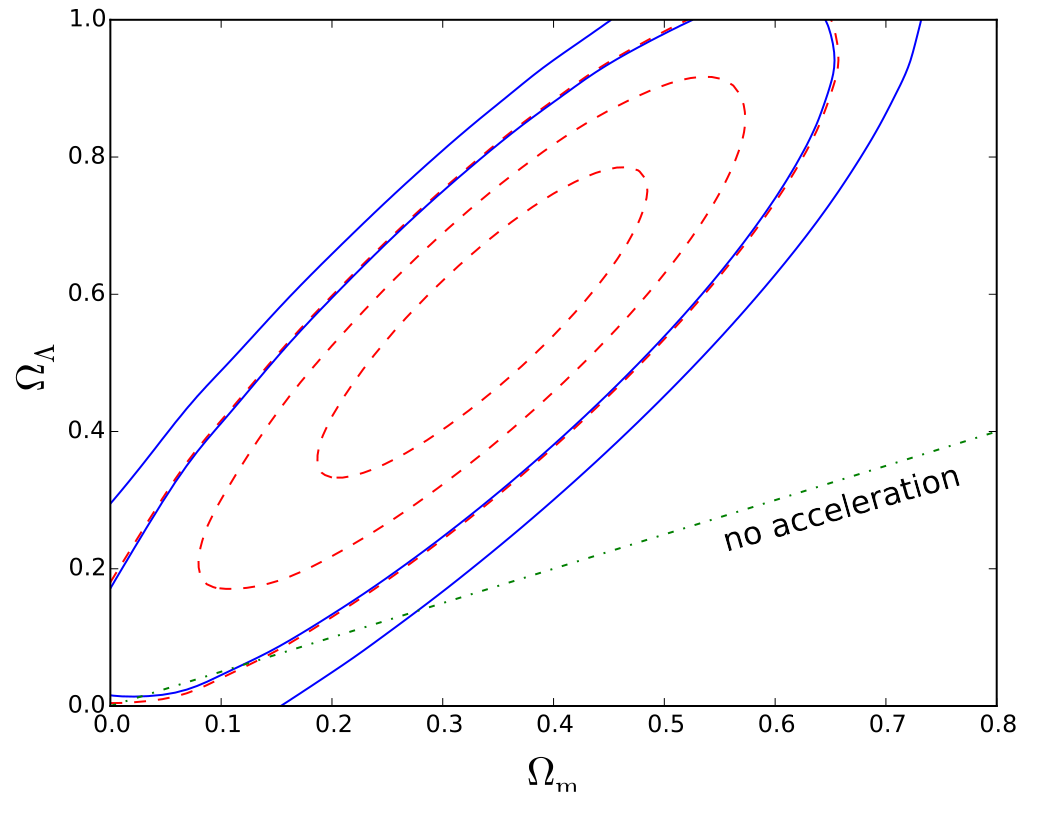
\includegraphics[width=0.7\textwidth]{./Pictures/sarkar_acceleration.png}
\caption{Reanalysis by J. T. Nielsen et~al. of the Nobel Laureate SNIa data, demonstrating that accelerated expansion is solid \cite{2016NatSR...635596N}.}
\label{fig:sarkar_SNIa}
\end{center}
\end{figure}

\section{Dark Energy Models}
Two independent experiments of different properties of the Universe show contradictory measurements: the Universe is flat and its expansion is accelerated. This implies two things, either \autoref{eq:einsteinbare} is wrong or the Universe is filled with new matter specie, that does not dilute with cosmic expansion and has negative pressure. Whatever drives this accelerated expansion is known as Dark Energy. Dark Energy models can be divided in three categories: the cosmological constant, exotic matter fields and modified gravity.
\newline

Among all the possible explanations, the cosmological constant is considered the fiducial explanation for dark energy.

\subsection{The Cosmological Constant}
The Cosmological Constant was initially proposed by Einstein himself \cite{1917SPAW.......142E} to avoid the solutions of the General Relativity where the Universe was not static and later discarded, when the expansion of the Universe was discovered by Hubble. Nevertheless, on the light of the recent events of accelerated expansion, the Cosmological Constant was soon recovered. The approach followed by this model consist on the addition of an additional covariant term to the Einstein field equations, a term proportional to the metric tensor ($\Lambda g_{\mu\nu}$), resulting \cite{2001LRR.....4....1C}:
\begin{equation}
R_{\mu\nu}-\frac{1}{2}Rg_{\mu\nu}+\Lambda g_{\mu\nu} = \frac{8\pi G_N}{c^4}T_{\mu\nu}.
\end{equation}
With this new term and assuming $\Omega_K=0$ \autoref{eq:flrw} transforms into
\begin{equation}
H^2(t) = H_0^2\left[\sum_i\Omega_i(t) +\Omega_\Lambda\right],
\end{equation}
where $\Omega_\Lambda$ is the dark energy critical density. This new term is a time-independent constant that has the same value on every location of the Universe. Thus, as the other matter species has a critical density that decreases with time, the dark energy critical density has only impact at late cosmic times.
\newline

This new term may be regarded as a new matter specie such that
\begin{equation}
\rho_\Lambda = \frac{3H_0^2}{8\pi G_N}\Omega_\Lambda.
\end{equation}
Taking into account \autoref{eq:conservationenergy}, an upper bound on the dark energy density can be established
\begin{equation}
\rho_v \leq \frac{3H_0^2}{8\pi G_N} \sim 10 ^{-47} \mbox{ GeV}^4.
\end{equation}
\newline

Since this energy density is fills the whole Universe and is an inherent property of the geometry of the Universe and hence of the Universe itself, from a physical point of view it can be identified as the energy of the vacuum \cite{RevModPhys.61.1,2003PhR...380..235P}. Quantum Field Theory (QFT) states that the quantum vacuum is not empty and static but it actually is a dynamical entity where particle and antiparticles are constantly produced and annihilated as it has been demonstrated by the Casimir effect. Energy density of the vacuum can be estimated
\begin{equation}
\rho_{QFT} = \int\limits_0^{1/L_P} dk \sqrt{k^2+m^2}\frac{4\pi k^2}{(2\pi)^4}\sim 10^{71}\mbox{ GeV}^4,
\end{equation}
where $L_P$ is Planck's length. Thus, there's a miss-match between the amount of dark energy measured and that predicted by QFT of several orders of magnitude. It can be argued that although it is known that Planck's energy scale is the upper range of validity of Standard Model physics, nothing prevents that it starts to fail at lower scales. A lower bound on this point can be established as the Quantum Cromodynamics (QCD) cutoff scale ($\sim 200$ MeV), leading to a vacuum energy density of
\begin{equation}
\rho_{QCD} = \int\limits_0^{1/L_{QCD}} dk \sqrt{k^2+m^2}\frac{4\pi k^2}{(2\pi)^4}\sim 10^{-3}\mbox{ GeV}^4,
\end{equation}
reducing the tension between theory and experiment, but still being catastrophic. Some theories claim that a cancellation of modes may arise at super-symmetry models. Nevertheless, latests LHC results excluded most of the phase-space of supersymmetric models \cite{2015arXiv150603091B}.
\newline

Several discrepancies indicate that either something is missing on the High Energy Physics side or on the Cosmology side. Nevertheless, it can be argued that no connection between the cosmological constant and quantum theory exists and define the cosmological constant as a free parameter of the theory. Despite this, a fine tune problem arises: the coincidence problem. As it has been observed by many experiments, the present day dark energy and matter density are very close, allowing the formation of structure. The redshift at which matter and dark energy densities are equal is given by
\begin{equation}
z_{eq} = \sqrt[3]{\frac{\Omega_\Lambda^0}{1-\Omega_\Lambda^0}}-1
\label{eq:equality}
\end{equation}
with $\Omega_\Lambda^0\in(0,1)$. Current measurements indicate that $\Omega_\Lambda^0\sim0.7$, demanding that $z_{eq}\sim0.3$. Those redshifts such that $z<z_{eq}$ are dominated by dark energy, inhibiting structure formation. The variation of \autoref{eq:equality} with dark energy density is not smooth and variations on this parameter lead to completely different results. An  increase of the 20\% on the dark energy density leads to a value of $z_{eq}=2.7$, preventing structure formation, whereas a decrease of the 20\% leads to $z_{eq}=-0.1$, indicating the universe is still matter dominated, preventing the detection of cosmic expansion. This fine tuning issue indicates that there must be some mechanism that couples dark energy and matter. Anthropic arguments can be made, stating that the value of the dark energy density has the value we measure since it is the only possible compatible with the detection of cosmic acceleration and structure formation.
\subsection{Exotic matter fields}
Since no satisfactory explanation has been found on the vacuum to explain dark energy, the presence on new quantum fields that, on the simplest case, interact only trough gravity, but on more complicated scenarios may also couple arbitrarily with the other matter fields can be considered.
\newline

The simplest case is known as quintessence and is defined as a scalar field that is added to the Lagrangian defined at \autoref{eq:einsteinbare} such that such that
\begin{equation}
\mathcal{L}[g_{\mu\nu}] = \sqrt{g}\left(g^{\mu\nu}R_{\mu\nu}(g)+\mathcal{L}_\phi\right)\ \ \mbox{ with }\ \ \mathcal{L}_\phi = -\frac{1}{2}g^{\mu\nu}\partial_\mu\phi\partial_\nu\phi-V(\phi),
\end{equation}
where $V(\phi)$ is the potential of the field. On an FLRW metric, this leads to a substance with density and pressure 
\begin{equation}
P_\phi = \frac{1}{2}\dot\phi^2-V(\phi)\ \ \mbox{ and }\ \ \rho_\phi=\frac{1}{2}\dot\phi^2+V(\phi).
\end{equation}
This can be parametrized as an ideal fluid with equation of state
\begin{equation}
w_{DE} = \frac{P_\phi}{\rho_\phi} = \frac{\dot\phi^2-2V(\phi)}{\dot\phi^2+2V(\phi)}.
\end{equation}
Thus, it can be deduced that dark energy critical density evolves with the scale factor of the universe as
\begin{equation}
\Omega_\Lambda(t) = \Omega_\Lambda^0 [a(t)]^{-3(1+w_\phi)}.
\end{equation}
\newline

The only possible candidate for dark energy as quintessence within the Standard Model of Particle Physics is the Higgs field, a complex scalar-field that fills the Universe and couples to gauge bosons giving them its mass. The potential of the field is given by
\begin{equation}
V(\phi) = \mu_H^2\phi^\dagger\phi+\frac{1}{4}\lambda_H(\phi^\dagger\phi)^2,
\end{equation}
with $\mu_H$ the mass term, $\lambda_H$ the self-interaction of the field and $\phi,\phi^\dagger$ the Higgs field and its hermitian conjugate respectively. Since the potential of the field is time independent, this leads to an equation of state
\begin{equation}
w_{DE} = \frac{-2V(\phi)}{2V(\phi)} = -1,
\end{equation}
recovering the cosmological constant solution. Thus, cosmological constant can be interpreted as the expected value of Higgs field at vacuum
\begin{equation}
\langle 0|\phi_0|0\rangle = \frac{|\mu_H|}{\sqrt{\lambda_H}}= \sqrt{\frac{1}{\sqrt{2}G_F}}= 246\mbox{ GeV},
\end{equation}
where $G_F$ is the Fermi constant, that can be computed from the decay of the muon. The connection between the decay of the muon and the Higgs field comes from the fact that the decay is mediated by vector bosons, whose mass is given by the Higgs field:
\begin{equation}
\mu^- \rightarrow W^- + \nu_\mu \mbox{ and }W^-\rightarrow e^-+\bar\nu_e.
\end{equation}
\newline

Other High Energy Physics scalar potentials can be built from physics beyond the Standard Model, such us supergravity \cite{1999PhLB..468...40B,1999astro.ph.12005B,2000PhRvD..61j3502B}, where a scalar potential can be found such that
\begin{equation}
V(\phi) = M^{4+n}\phi^{-n},\exp(\alpha\phi^2/m^3_P),
\end{equation}
which has a minimum with $w_{DE}\simeq -0.8$, close to the cosmological constant value. Within a supersymmetry breaking framework, a field with potential 
\begin{equation}
V(\phi) = M^{4+n}\phi^{-n}
\end{equation}
can be introduced \cite{1999PhRvD..60f3502B}. Nevertheless most of the phase space of supersymmetry and supergravity has been excluded by latest LHC results.
\newline

The existence of an ultra-light Pseudo-Nambu-Goldstone Boson may be postulated with an associated field with potential \cite{PhysRevLett.75.2077,1992PhRvD..45.2674F}
\begin{equation}
V(\phi) = M^4\cos^2(\phi/f).
\end{equation}
Light-massive Pseudo-Nambu-Goldstone Bosons can be found as exotic forms of matter such as axions and schizons, whose existence is far from being probed.
\newline

More complicated field models can be considered increasing the number of fields and letting them interact and will not be considered here since they are beyond the scope of this Thesis. A detailed description of all the models can be found at \cite{2010deto.book.....A}. Nevertheless, a general phenomenological description can be made in terms of the equation of state of dark energy,
\begin{equation}
P_{DE} = w_{DE}\rho_{DE}
\end{equation}
expanding the parameter $w_{DE}$ in a power series of the scale factor
\begin{equation}
w_{DE}(t) = w_0 +w_a[1-a(t)],
\end{equation}
where $w_0$ denotes the value of the equation of state parameter at present and $w_a$ is evolution --at first order-- with time. The cosmological constant may be considered as an specific solution of this equation of state where
\begin{equation}
w_0=-1\ \ \mbox{ and }\ \ w_a=0.
\end{equation}

\subsection{Modified Gravity}
Attempts to explain the existence of a cosmological constant from High Energy Physics side, leads to a tension between General Relativity and the Standard Model. Possible new exotic fields that may explain late-time cosmic acceleration are walking a tightrope due to latest LHC results from physics beyond the Standard Model.
\newline

The remaining approach to explain the accelerated expansion of the Universe is to consider General Relativity as an approximate gravitational theory on the same way Newtonian gravity is the low-energy limit of Einstein's gravity. Extensions to General Relativity are known as modified gravity models. This kind of models were born as alternate theories to dark matter as explanation of Vera Rubin's measurements of the rotation curve of spiral galaxies \cite{1982ApJ...253...70B,1983Sci...220.1339R,1985ApJ...289...81R,1985ApJ...297..423B}. 
\newline

The first theory is Milgrom's Modified Ordinary Newtonian Dynamics (MOND)  and its relativistic extensions \cite{1983ApJ...270..365M,1984ApJ...286....7B,1997ApJ...480..492S,1994ApJ...429..480B}, that suggest that Newton's second law is not valid on galactic scales, not requiring the existence of dark matter. Although some tests on galactic scales support MOND \cite{2011PhRvL.106l1303M,2013PhRvL.111d1105M}, this paradigm can not explain the Bullet Cluster \cite{2006ApJ...648L.109C,2006ApJ...652..937B,2007MNRAS.382...29B} (see \autoref{fig:bullet}). Recently Verlinde proposed a new theory that postulates gravity as a consequence of quantum entanglement at the microscopic level \cite{2016arXiv161102269V}. Although, this theory recovers MOND results for point masses, it has been rapidly put in tension with the measurement of the rotation curve of galaxies \cite{2017MNRAS.468L..68L}.
\begin{figure}
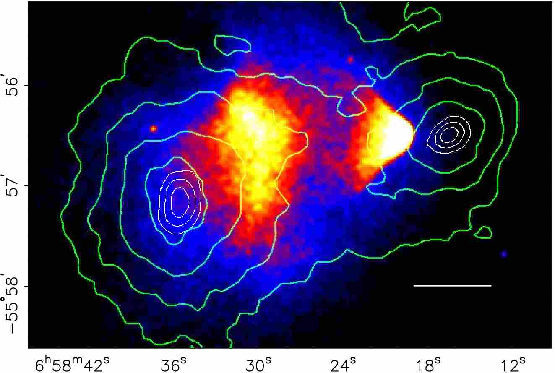
\includegraphics[width=\textwidth]{./Pictures/bullet_cluster.png}
\caption{Bullet cluster. Colors indicate the barionic mass measured with gamma-rays, whereas the solid lines indicate the mass reconstructed with gravitational lensing. This result is considered the clearest probe of the existence of dark matter and that it is decoupled from barionic matter. Image taken from \cite{2008PhRvD..78j4004D}.}
\label{fig:bullet}
\end{figure}
\newline

More elaborated theories that do not break the equivalence principle can be made. One class of those theories is known as $f(R)$ gravity \cite{2010LRR....13....3D,2010RvMP...82..451S}, and its approach is to let the Lagrangian to be a general function ($f$)
of the Ricci scalar, $R=g^{\mu\nu}R_{\mu\nu}$:
\begin{equation}
\mathcal{L}[g_{\mu\nu}] = \frac{c^4}{16\pi G_N}\sqrt{-g}f(R),
\end{equation}
that leads to the field equation
\begin{equation}
R_{\mu\nu}-\frac{1}{2}Rg_{\mu\nu}=\frac{8\pi G_N}{c^4}( T_{\mu\nu}+T_{\mu\nu}^R).
\end{equation}
This field equation is similar to \autoref{eq:einsteinbare} but has an additional term $T_{\mu\nu}^R$ that takes into account the additional curvature terms that can be modeled as a fluid on the same way as the energy-momentum tensor. The simplest case is $f(R) =R+\alpha R^n$ with $\alpha,n\in\mathbb{R}$. It has interesting cosmological solutions \cite{PhysRevD.85.083511}, nevertheless the latest studies on the large-scale-structure of the Universe, favor $\Lambda$CDM over $f(R)$ models \cite{2013PhRvD..88d4050A} although a range of $n$ can not still be fully discarded. This theory has very distinctive phenomenology such as double Einstein rings on the strong lensing regime \cite{2011PhRvD..83b4030N} that --if found-- could be the smoking gun of these kind of theories.
\newline

More complicated models of modified gravity can be considered but are not going to be treated here since they are beyond of the scope of this Thesis. For a review it can be consulted \cite{2015CQGra..32x3001B}. The usual approach to explore the modifications to General Relativity \cite{2015PhRvD..91h3504L} are to model the departures of the metric. On the Newtonian gauge, the FLRW line element of can be parametrized with the Newtonian and the lensing potential; $\Phi,\Psi$ respectively \cite{2015PhRvD..91h3504L}:
\begin{equation}
ds^2 = a^2(\tau)[-(1+2\Phi)d\tau^2+(1-2\Phi)dx_idx^j],
\end{equation}
with
\begin{equation}
2\nabla^2\Phi(a,k) = \frac{8\pi G_N}{c^2}a^2\mu(a,k)\bar \rho_M\delta_M(a,k)\ \ \mbox{ and }\ \ \gamma(a,k)=\frac{\Phi(a,k)}{\Psi(a,k)},
\end{equation}
where $\bar \rho_M$ is the average matter density, $\delta_M$ its fluctuations and $k$ is the wavenumber of the potentials. Here $\mu$ and $\gamma$ parametrize the departures from General Relativity, that is the specific case with
\begin{equation}
\mu(a,k) = 1\ \ \mbox{ and }\ \ \gamma(a,k) = 1.
\end{equation}

It is important to remark that the zoo all the departures from General Relativity plus cosmological constant --including the addition of new fields--, may be unified into a single parametrization known as Parametrized Post-Friedmann Framework \cite{2013PhRvD..87b4015B}.

\section{Current status of Dark Energy constrains}
The latest and more precise results constraining dark energy are provided by the Planck Collaboration 2015 results from the analysis of the Cosmic Microwave Background (CMB) \cite{2016A&A...594A..14P}.
\newline

Dark enery as an exotic form of matter, is determined by measuring the parameters of the equation of state ($w_0,w_a$) and their value can be seen at \autoref{fig:w0wa_planck2015}. The results provided are compatible with General Relativity plus cosmological constant, the uncertainty on the parameters of the equation of state does not allow to exclude many models, specifically the type of models that predict a value of the equation of state close to that of the cosmological constant but whose equation of state evolves with cosmic time --or equivalently, redshift--, since current precision on the determination of this evolution is still very poor as it can be deduced from \autoref{fig:equationofstate_planck2015}. Constrains on Modified Gravity models are also given in terms of the modified gravity potentials $\mu,\eta$ and $\Sigma$. As it can be deduced from \autoref{fig:mg_planck2015} and \autoref{fig:munu_planck2015}, General Relativity plus cosmological constant is not excluded but, as in the case of the fluid equation, the measurements are not precise enough to discard many modified gravity models.
\newline

\begin{figure}
\begin{center}
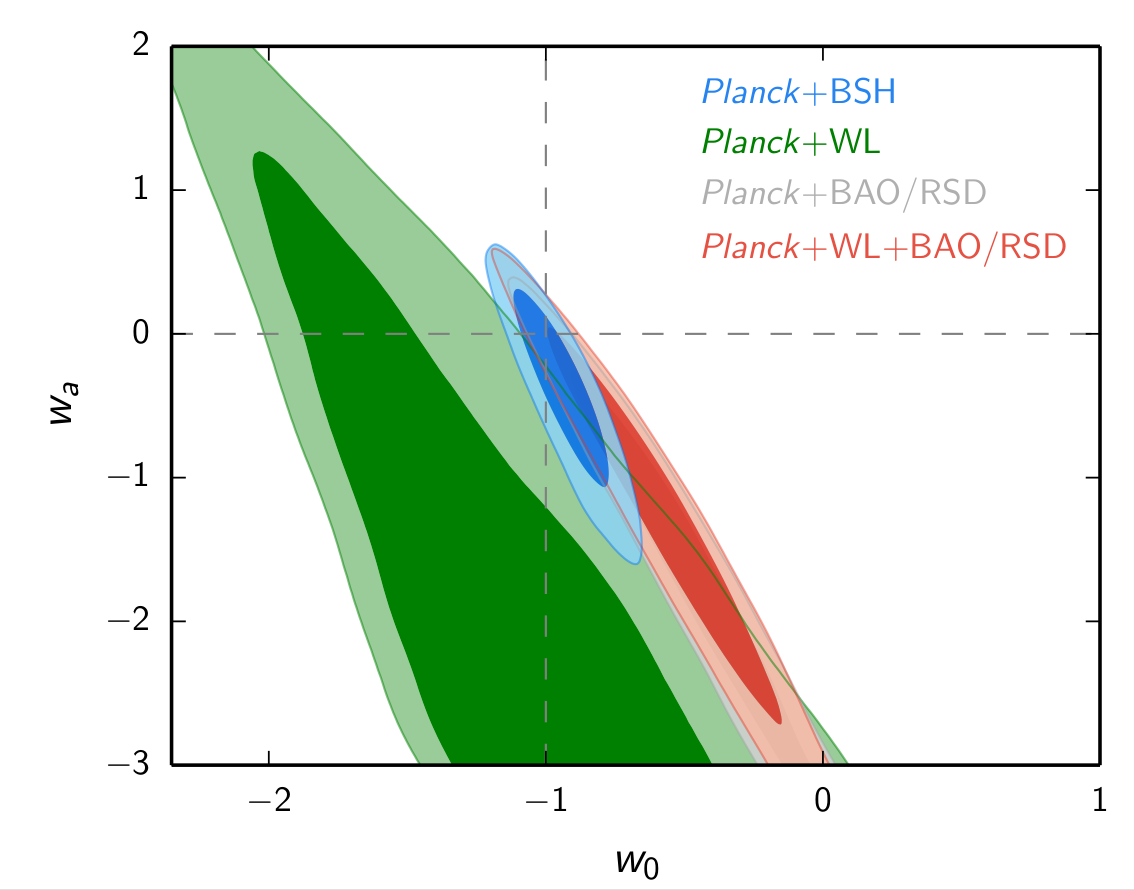
\includegraphics[width=0.8\textwidth,trim={0 3mm 0 0},clip]{./Pictures/w0wa_planck2015.png}
\caption{One- and two- sigma contours of the equation of state of dark energy $w_0,w_a$. The intersection of dashed lines is the cosmological constant. Results obtained from Planck Collaboration 2015 results \cite{2016A&A...594A..14P}.}
\label{fig:w0wa_planck2015}
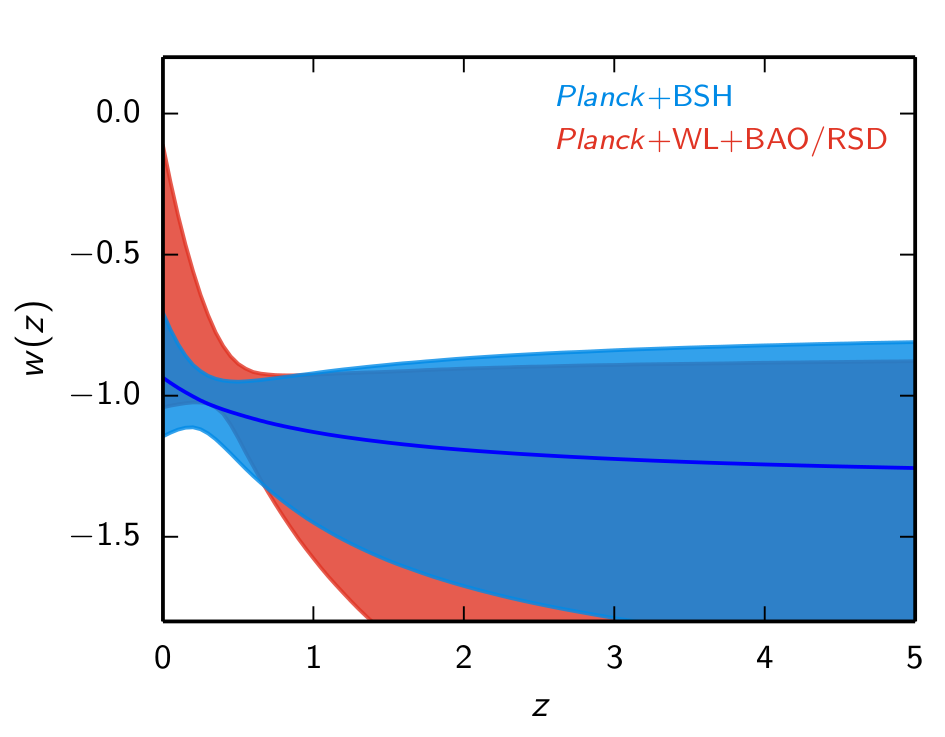
\includegraphics[width=0.8\textwidth]{./Pictures/equationofstate_planck2015.png}
\caption{One-sigma confidence interval of the equation of state of dark energy as a function of redshift $w_{DE}(z)$ and one-sigma confidence interval. Results obtained from Planck Collaboration 2015 results \cite{2016A&A...594A..14P}.}
\label{fig:equationofstate_planck2015}
\end{center}
\end{figure}

\begin{figure}
\begin{center}
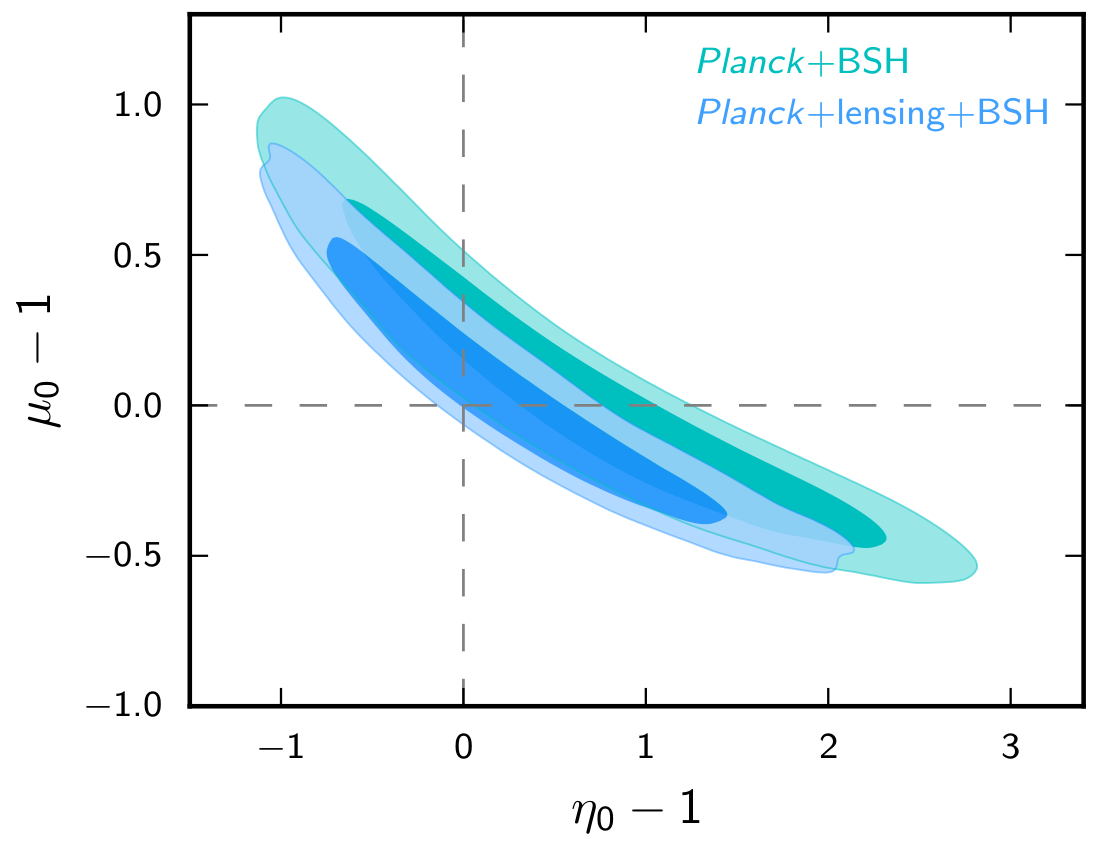
\includegraphics[width=0.8\textwidth]{./Pictures/mg_planck2015.png}
\caption{One- and two- sigma modified gravity potentials at present $\mu_0,\eta_0$. Dashed line is General Relativity plus cosmological constant. Results obtained from Planck Collaboration 2015 results \cite{2016A&A...594A..14P}.}
\label{fig:mg_planck2015}
\vspace*{0.2cm}
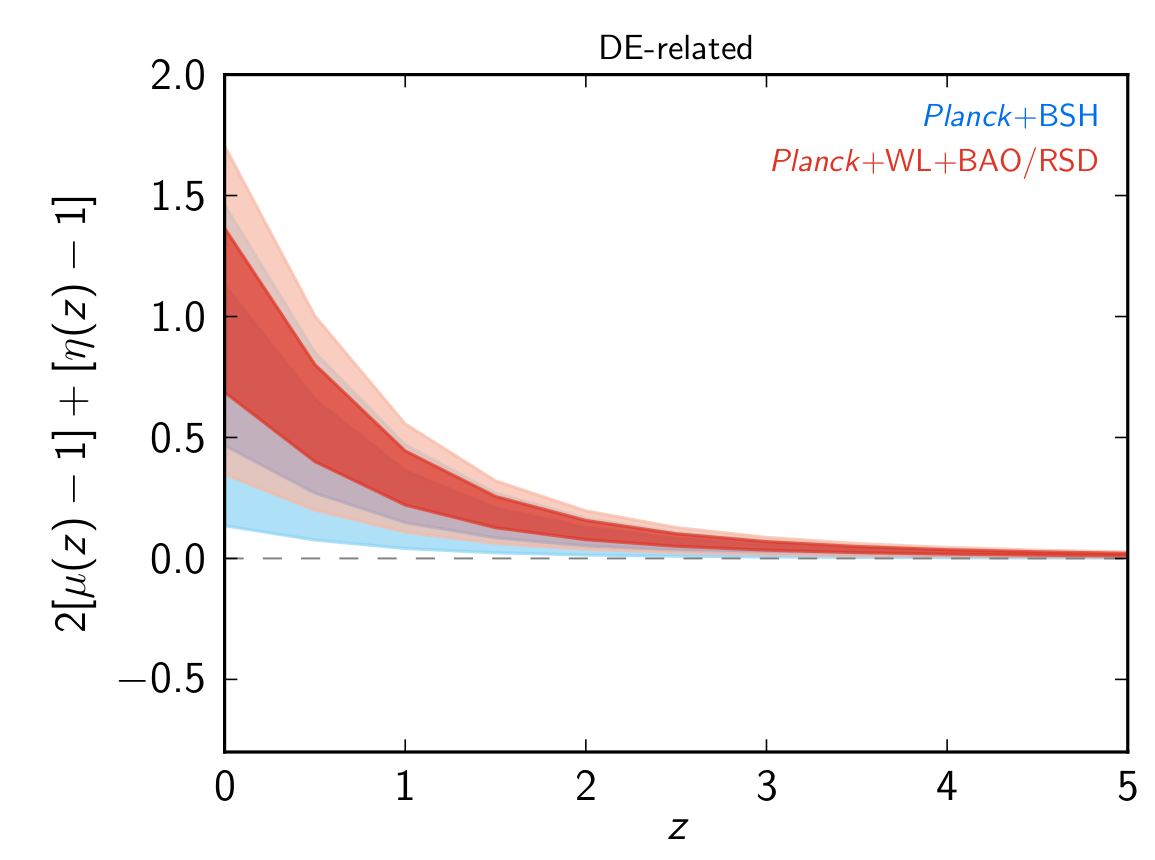
\includegraphics[width=0.8\textwidth]{./Pictures/munu_planck2015.png}
\caption{One- and two- sigma of the sum of the modified gravity potentials. Dashed line is General Relativity plus cosmological constant. Results obtained from Planck Collaboration 2015 results \cite{2016A&A...594A..14P}. }
\label{fig:munu_planck2015}
\end{center}
\end{figure}

Although the Planck Collaboration 2015 results seems to favor cosmological constant as dark energy, Riess et~al. latest direct determination of the Hubble constant using the cosmological distance ladder (parallax-cepheids-SNIa) \cite{2016ApJ...826...56R}, show a discrepancy on the $3\sigma$ level with the Hubble constant measured by Planck Collaboration 2015. If more exotic cosmological scenarios are considered, such as non-flatness, additional species of neutrinos or other models of dark energy are allowed, this tension is relaxed. 
\newline

CFHTLens \& KiDS-450 Collaborations galaxy-shear weak-lensing analysis show tension on the $\Omega_M-\sigma_8$ plane with Planck Collaboration 2013 \cite{2014A&A...571A..16P} and 2015 CMB measurements if a General Relativity plus cosmological constant scenario is considered \cite{2013MNRAS.430.2200K,2017arXiv170303383H}. This tension may be alleviated if other models are considered, such as non-zero curvature and dark energy models \cite{2016arXiv161004606J}. Nevertheless, discrepancies could also be produced by systematic effects \cite{2015PhRvD..92b3003D,2017MNRAS.465.2033J}.
\newline

A weak-lensing analysis by Leauthaud et~al. \cite{2017MNRAS.467.3024L} of CFHTLens \& CMASS data using gg-lensing show a lower signal amplitude that the one predicted measuring the clustering of the lens sample. In addition gg-lensing measurements on the $\Omega_M^0-\sigma_8$ plane have a discrepancy on the $3\sigma$ level with Planck Collaboration 2013 measurements on a cosmological constant scenario. Nevertheless, discrepancies are interpreted in terms of new physics on the astronomy side: halo occupation distribution (HOD) and barionic physics.
\newline

As it has been described, current individual constrains on dark energy are not precise enough to determine which model is the correct explanation of the accelerated expansion of the Universe. Current cosmological model --General Relativity with flat geometry plus cosmological constant (flat-$\Lambda$CDM)--, is in crisis since a tension exists between different probes \cite{2016PDU....12...56B}. Dark energy is one of the possible scenarios to solve this tension, although caution is needed and analysis need to put special attention to systematic analysis. This requires additional probes and redundant measurements of the same physical observable but with different sources of systematic errors.


\section{Alternative probes for Dark Energy: Voids \& Troughs}
Previous cosmological probes were based on the same physical quantity: the anisotropies of the matter density-field although at different moments of the Cosmic History. Whereas CMB measures anisotropies at decoupling, lensing and clustering measure them at present. This anisotropies where originated on primordial density fluctuations\footnote{The current hypothesis suggests that this fluctuations are due to inflation.} that, when matter and radiation decoupled, froze. Then, the over-dense regions of the mater field started to grow by gravitational collapse of the matter, leading the the accretion of the matter contained at the under-dense regions, forming the cosmic  web (see \autoref{fig:2df}). This large under-dense regions of the Universe surrounded by over-dense regions are known as voids.
\begin{figure}
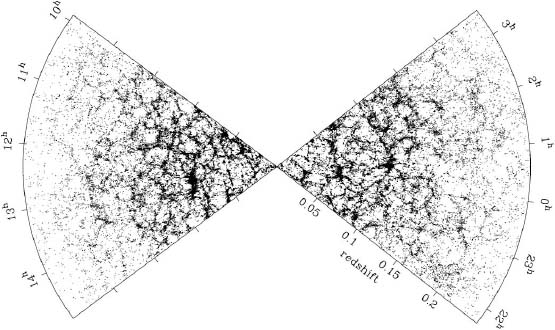
\includegraphics[width=\textwidth]{./Pictures/2df.jpg}
\caption{Large-scale-structure of the Universe. Each dot represents the position of a galaxy. Image credit: 2 Degree Field Survey.}
\label{fig:2df}
\end{figure}
\newline

Since voids have a lower matter content than the average Universe, their gravitational evolution is dominated by dark energy. Thus, void properties are different depending on the dark energy theory that rules the Cosmos. If the abundance of large voids on the Universe is considered, it has been reported that its number increases in $f(R)$ gravity models \cite{2012MNRAS.421.3481L} since the abundance of dark matter halos is altered \cite{2017JCAP...03..012V}. Nevertheless, if the shape of the void is measured, its ellipticity can be used as a probe for the parameters of the equation of state of dark energy \cite{2010MNRAS.403.1392L,0004-637X-754-2-109,PhysRevLett.98.081301,2013PhRvL.111x1103S}, since the structure growth-factor on the line-of-sight has a variation due to
the dark energy content, whereas on the transverse plane, growth-factor is constant. Finally, the radial distribution of matter around the center of a void --known as void profile-- has demonstrated to be different on $f(R)$ theories and General Relativity \cite{2014APh....54...44A,2014arXiv1410.8355C,2015MNRAS.451.4215Z,2015JCAP...08..028B,2016PhRvD..93j3522A,2016PhRvD..94j3524A}. Thus, by simply measuring the void matter profile, constrains on dark energy can be made.
\newline

Nevertheless, the total matter budget of the Universe is composed by both barionic and dark matter, being the presence of the latter only accessible indirectly trough its gravitational effects. As galaxies --mainly composed by barionic matter-- are biased tracers of the underlying dark matter field, its spatial distribution requires a model of assembly of galaxies within dark matter, introducing uncertainties and nuisance parameters on the model. Gravitational light deflection is only sensitive to the total matter field, not needing additional modeling on how barionic and dark matter relate. Thus, gravitational light deflection made by voids constitutes a promising new probe on dark energy.
